% Das gesetzt von Conway [Seite 39 EWolff2016:Microservices]
\chapter[Allgemeine Grundlagen]{Allgemeine Grundlagen zur Verwendung von Service-orientierten Systemen}
\label{chap:grundlagen}
Software zu entwickeln ist nicht immer einfach. Umso größer diese ist, umso mehr Probleme können auftreten. Es bedarf einer genauen Planung und Verständnis von Infrastruktur um eine Software mit allen Anforderungen zufriedenstellend zu implementieren. 

Vor allem wenn es um die Weiterentwicklung und Wartung von Software geht, können große Probleme auftreten. Wurde die Architektur nicht gut gewählt oder schlecht umgesetzt, kann es das weitere Vorgehen stark beeinträchtigen, bis hin zum unmöglich machen. Es wurden daher Software-Architekturen entwickelt, welche flexibel und einfacher zu ändern sind. Außerdem kann in diesen Architekturen neue Funktionen deutlich schneller hinzugefügt werden.

\section{Architektur}
\label{sec:architektur}
Microservice-Architekturen und \SOA (SOA) Architekturen können, wenn sie richtig angewendet werden, sehr flexibel und schnell änderbar sein. Beide Architekturen zielen, wie der Name schon sagt, auf eigenständige Services ab, welche durch verschiedene Kommunikationskanäle miteinander kommunizieren und dadurch die gewünschten Geschäftsprozesse abbilden. "Ein Programm soll nur eine Aufgabe erledigen, und das soll es gut machen" \cite[S. 2]{EWolff2015:ContinuouosDelivery}. Anstatt eine einzige große Anwendung ein zu setzten, setzt man auf viele kleine, verteile, autarke Anwendungen, welche jeweils Schnittstellen nach außen hin anbieten damit der Service genutzt werden kann. Diese Schnittstellen können unter anderem durch REST-HTTP angeboten werden.
Durch die verteilten Anwendungen funktioniert das System auch dann noch, wenn einzelne Services nicht verfügbar sind, jedoch bringt es ebenfalls die typischen Probleme von Verteilten Anwendungen mit sich, welche in \secref{chap:fallstudie} noch genauer erläutert werden.
\\\\
\textbf{Services kann man in drei Kategorien einteilen:}
\begin{description}
    \item[Producer] Ein Service der etwas Produziert oder auf eine Anfrage reagiert. Das reicht von Daten aus einer Datenbank extrahieren bis hin zu komplexen Berechnungen.
    \item[Consumer] Ein Service oder eine Anwendung, welche einen oder mehrere Produzierende Services verwendet und entweder weiterverarbeitet oder ausgibt. Im Falle der Weiterverarbeitung ist ein Consumer ebenfalls ein Producer sein.
    \item[Self-Contained System (SCS)] "\frqq Microservice mit UI\flqq\ oder \frqq Self-Contained System\flqq\ wie es Stefan Tilkov nennt, sind in sich abgeschlossene Systeme. [..] Sie enthalten eine UI und sollten möglichst nicht mit anderen SCS kommunizieren." \cite[vgl S. 55]{EWolff2016:Microservices}. SCS sind jedoch nur im Microservice und nicht im SOA Umfeld zu finden. Warum wird in \secref{chap:fallstudie} weiter erläutert.
\end{description}

\subsection{Das Gesetzt von Conway}
\label{subsec:conway}
Wie in \cite[S. 39 ff.]{EWolff2016:Microservices} beschrieben, stammt das Gesetzt von dem amerikanischen Informatiker Melvin Conway und besagt:
\begin{center}
    \textit{Organisationen, die Systeme designen, können nur solche Designs entwerfen, welche die Kommunikationsstruktur dieser Organisationen abbilden.}
\end{center}
"Conway möchte damit ausdrücken, dass die internen Kommunikationswege wichtig bei der Planung der Architektur ist. Jedes Team innerhalb einer Organisation trägt bei der Entwicklung der Architektur bei. Wird eine Schnittstelle zwischen zwei Teams benötigt, so müssen diese Teams auch kommunizieren können. Dabei müssen Kommunikationswege nicht immer offiziell sein. Oft gibt es informelle Kommunikationsstrukturen, die ebenfalls in diesem Kontext betrachtet werden können." \cite[vg. S. 39]{EWolff2016:Microservices}

\subsection{Domain-Driven Design und Bounded Context}
\label{sec:boundedContext}
Arbeitet man mit Service-Orientierten Architekturen, versucht man Services, welche zu einem bestimmten Kontext gehören, möglichst nahe beieinander zu halten. Man spricht hierbei von \textit{Bounded Context}. "Bounded Context ist ein zentrales Muster in Domain-Driven Design.[..] DDD arbeitet mit großen Modellen, indem es diese in kleine verschiedene zusammengehörige Kontexte unterteilt und auf ihre Wechselwirkung unterteilt."\cite{mfowler:BoundedContext}

\begin{figure}[htb]
    \centering 
    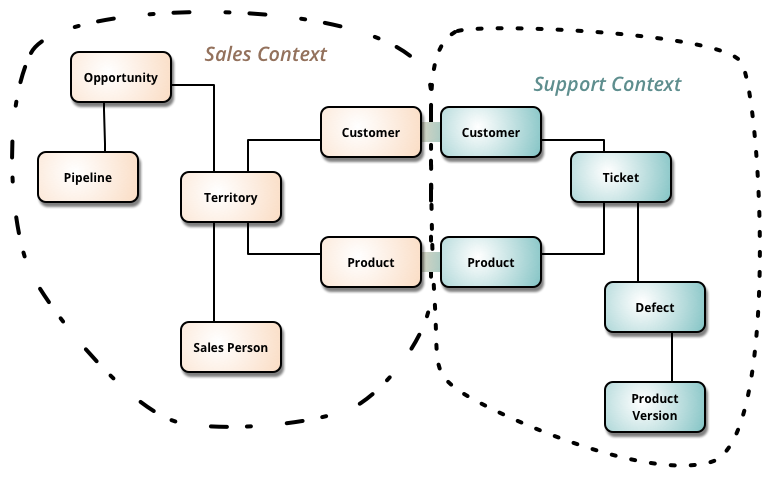
\includegraphics[width=\linewidth]{content/images/BoundedContext}\
    \quelle\url{http://martinfowler.com/bliki/BoundedContext.html}
    \caption[Bounded Context]{Bounded Context\\}
    \label{fig:BoundedContext}  
\end{figure}\noindent  
In dieser Grafik wird noch einmal der Begriff Bounded Context genauer verdeutlicht. Es existieren zwei eigenständige Prozesse. Auf der linken Seite der Sales Kontext und auf der rechten Seite der Support Kontext. Jeder Kontext besitzt verschiedene Services, welche benötigt werden um den Prozess durchführen zu können. Lediglich zwischen den \textit{Customer} und \textit{Product} Services besteht eine Verbindung der beiden Prozesse.

\section{Werkzeuge}
\label{sec:werkzeuge}
Anders als bei Monolithischen-Projekten, bestehen Service-Orientierte-Projekte aus vielen kleinen Services, die alle einzeln verwaltet werden müssen. Das sie laufen reicht nicht aus, sie müssen auch geupdated und gewartet werden.

Im folgenden sollen daher einige Werkzeuge vorgestellt werden, welche das bauen, prüfen, ausliefern und verwalten der einzelnen Services vereinfacht und automatisiert. Einige dieser Werkzeuge werden für die Umsetzung, der in \secref{sec:ausgangssituation}\ vorgestellten Anforderung, eingesetzt und in dem dafür vorgesehenen Kapitel weiter erläutert.

\subsection{Jenkins}
\label{subsec:jenkins}
Jenkins ist ein in Java geschriebenes, webbasiertes Software-System, für \ci\ (CI) \ \cd\ (CD). Es kann unter anderem durch Plugins um weitere Funktionen erweitert werden. Mit Hilfe von Jenkins sollen das Bauen, Testen und Ausliefern automatisiert werden.\footnote{\cite[vgl. S. 98 ff.]{EWolff2015:ContinuouosDelivery}}

\subsection{Puppet}
\label{subsec:puppet}
Puppet ist ein Systemkonfigurationswerkzeug. Es soll durch Konfigurationsdateien eine Standardisierte Installation von Software ermöglichen. Über ein Master-Slave System können diese dann via Netzwerk auf mehreren Computern/Servern verteilt werden.

\subsection{Docker}
\label{subsec:docker}
Docker soll die Auslieferung von Anwendungen vereinfachen, in dem die Anwendung in ein Container isoliert wird. Die so entstehende Datei wird Image genannt. Zum Ausliefern der Anwendung reicht es, wenn das Image an den jeweiligen Bestimmungsort kopiert und dort ausgeführt wird. Das kann zum Beispiel durch Puppet geschehen. Dies ermöglicht außerdem, dass eine Anwendung auf verschiedenen Servern exakt gleich ausgeführt wird.
Docker setzt dabei auf Linux Container. Dadurch ist nur eine Instanz des Kernels im Speicher, jedoch sind die Prozesse, Benutzer, Dateisystem und Netzwerk von einander getrennt. Das ermöglicht außerdem, dass mehrere Docker Images zusammen arbeiten.\footnote{\cite[vgl. S. 53 ff.]{EWolff2015:ContinuouosDelivery}}

\subsection{Vagrant}
\label{subesec:vagrant}
Mit Hilfe von Vagrant kann man einfach und schnell Virtuelle Maschinen standardisiert aufsetzten. Dabei nutzt das Werkzeug fertige Betriebssystem Images, wie sie zum Beispiel mit VirtualBox erstellt werden können. Die Virtuelle Maschine wird durch das sogenannte Vagrantfile konfiguriert. Innerhalb dieser Datei kann zum Beispiel mit Puppet zusätzliche Software installiert werden. Dadurch kann schnell ein neues Produktiv- oder Testsystem aufgebaut werden.
\footnote{\cite[vgl. S. 49 ff.]{EWolff2015:ContinuouosDelivery}}

\subsection{Swagger}
\label{subsec:swagger}
Die bisherigen Werkzeuge dienten dazu, Services auszuliefern, aber sie müssen, wie bereits weiter oben erwähnt, Schnittstellen anbieten, damit sie genutzt werden können. Diese müssen jedoch auch dokumentiert sein, damit ein Entwickler weiß, welche Schnittstelle er wie anzusprechen hat. Durch Swagger ist eine einfache und zentrale Dokumentation von REST-HTTP Schnittstellen möglich.

\subsection{Service Discovery}
\label{subsec:ServiceDiscovery}
Mit Swagger haben wir die Schnittstellen dokumentiert, jedoch kann es bei vielen Services problematisch werden, den richtigen zu finden. Dafür sind sogenannte Service Discovery Werkzeuge wie Spring Eureka von Netflix oder Apache Zookeeper zuständig. Sie können außerdem dafür sorgen, dass ein Programm automatisch einen anderen Server bekommt, wenn ein genutzter Service ausfallen sollte. \footnote{\cite[vgl. S. 326 ff.]{EWolff2016:Microservices}}

\subsection{ELK (ElasticSearch, LogStash, Kibana)}
\label{subsec:elk}
Durch Service-Orientierte Systeme gibt es viele verteilte Anwendungen. Um sie zu warten und Fehler beheben zu können, müssen die Protokoll Dateien ausgewertet werden. Da jedoch die Services im Netzwerk verteilt sind, sind auch die Protokolle verteilt. Durch den ELK-Stack ist ein einheitliches Logging möglich.
Mit Hilfe von \textit{Logstash} können die Log-Dateien im von Servern im Netzwerk eingesammelt und mit \textit{Elasticsearch} zentral gespeichert werden. \textit{Kibana} ist eine Weboberfläche, mit der die gespeicherten Protokoll Daten in ein für Menschen leserliches Format angezeigt und ausgewertet werden kann.
\footnote{\cite[vgl. S. 244 ff.]{EWolff2016:Microservices}}